\chapter{仿真时间奖励}

\section{工作原理}
在对物理过程进行仿真的过程中,物理引擎往往会做一些缓存和优化来对仿真进行加速,而这种加速是基于此物理过程容易预测这一事实的。这意味着,对于难以进行预测的复杂物理行为,如复杂的碰撞,物理引擎要消耗更多的时间来进行仿真。这就使得利用此信息来为智能体提供任务无关的探索奖励成为可能。

在实验过程中,为了准确计算仿真时间,避免其他因素影响,必须保证在训练过程中没有其他程序在运行。这一要求可以简单地通过避免在训练时操作计算机来满足。此外,为了防止系统调用的时间被计入,在实验中对仿真时间进行计算时,直接在仿真代码被调用前后使用Python的time库进行了计时。

除了仿真时间奖励外,实验中还提供了基于局部敏感哈希的探索奖励。为了平衡不同的内部奖励,需要在计算最终奖励前先乘上一个系数。

在演员网络中,使用了上一章提出的混合高斯噪声层,但不同的是,为了防止噪声产生过大影响,继续使用参数$\sigma_{clip}$对噪声进行裁剪。

为了防止机械臂在可以完成任务的动作序列中选择较长的序列,在对演员网络进行优化时,可以在其损失函数中添加一个动作正则化项,即

   $$ L_\mu = -\sum_i^N\frac{Q_1(s_i, \mu(s_i))}{N} + \xi_{action}||\mu(s_i)||^2$$
其中$\xi_{action}$是动作正则化系数。

在实验中,整个系统都采用\ref{myenvexp}中的设计,但是除了使用\ref{myenvexp}中的浅层网络结构外,还增加了一个为每个网络添加一个隐藏层的深层网络作为对照组。

由于在使用正向动力学预测模型来计算奖励时,会导致训练速度极大下降,而且在实验中并未发现它能够对算法结果产生有利影响,因此在本章实验中不再展示相关的实验结果和数据。

实验相关的参数见表\ref{simtable}。
    \begin{table}[htbp]
        \caption{仿真时间奖励实验参数}
        \label{simtable}
    \vspace{0.5em}\centering\wuhao
    \begin{tabular}{ccccc}
    \toprule[1.5pt]
    实验参数 & 值\\
    \midrule[1pt]
        $\sigma_{clip}$ & 0.5\\
        $M$ & 300\\
        $\epsilon_{rand}$ & 0.3\\
        $\xi_{action}$ & $1\times 10^{-3}$\\
        $\gamma$ & 0.998\\
        $\alpha$ & $1\times 10^{-3}$\\
        $B$ & 256\\
        $\tau$ & 0.23\\
        $T$ & 200\\
        $N_{batches}$ & 4\\
        $f_{target}$ & 200\\
        $f_{actor}$ & 400\\
        $f_{critic}$ & 200\\
        $T_{start}$ & $1\times 10^5$\\
        $N_{sample}$ & 50 \\
        $k$ & 18\\
        $K_{replay}$ & 4\\
        $\xi_{LSH}$ & $2\times 10^{-2}$\\
        $\xi_{sim}$ & 10\\
    \bottomrule[1.5pt]
    \end{tabular}
    \end{table}
    其中$\xi_{action}$是动作正则化系数,$N_{batches}$指每次触发对演员网络或评论家网络的训练时迭代的次数。
    每经过$f_{target}$个时间步,使用指数滑动平均对靶网络进行权重更新。
    每经过$f_{actor}$个时间步,使用反向传播对演员网络权重进行更新。
    每经过$f_{critic}$个时间步,使用优化器对评论家网络权重进行更新。
    $\xi_{sim}$是在计算最终奖励时,仿真时间奖励的系数。
    其余的参数意义与表\ref{fcntable}中相同。
\section{实验结果与分析}

只有3层与有4层的网络相比,演员网络损失曲线如图\ref{simlossmu}所示。可以看出浅层网络更快地收敛了,而深层网络收敛到了一个损失较大的值。
        \begin{figure}
        \centering
        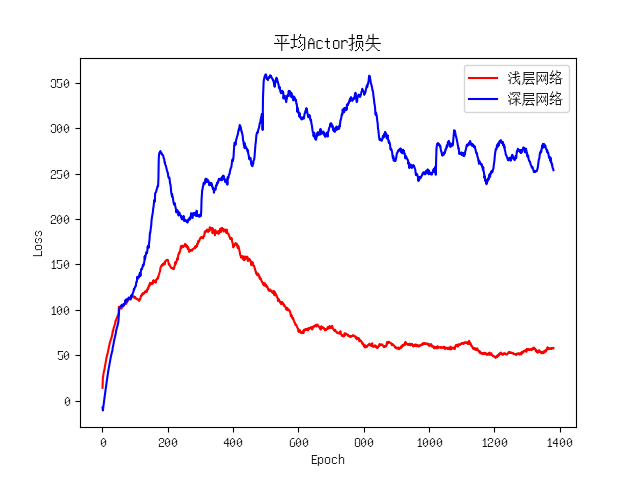
\includegraphics[width=0.6\textwidth]{sim_myenv_lossmu.png}
        \caption{3层和4层演员网络$\mu$的损失曲线}
            \label{simlossmu}
        \end{figure}

对于评论家网络来说,如图\ref{simlossq1}和\ref{simlossq2}所示,情况是类似的,更加值得注意的是,深层网络更容易出现损失突然暴增的现象,这意味着深层网络训练起来更加不稳定。
        \begin{figure}
        \centering
        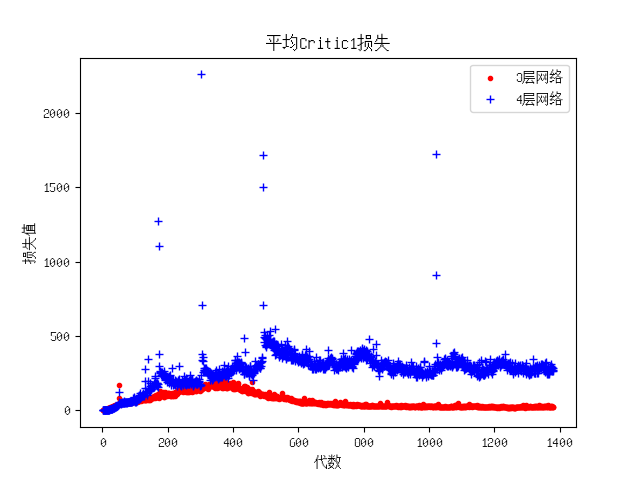
\includegraphics[width=0.6\textwidth]{sim_myenv_lossq1.png}
        \caption{3层和4层评论家网络$Q_1$的损失曲线}
            \label{simlossq1}
        \end{figure}

        \begin{figure}
        \centering
        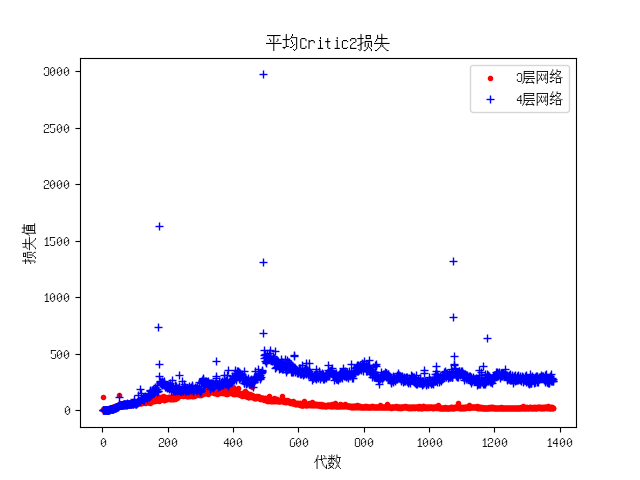
\includegraphics[width=0.6\textwidth]{sim_myenv_lossq2.png}
        \caption{3层和4层评论家网络$Q_2$的损失曲线}
            \label{simlossq2}
        \end{figure}

浅层网络和深层网络的平均环境奖励如图\ref{simenv_reward}所示,可以看出浅层最后学习到了一个较好的策略,得到的奖励显著比深层网络更高,而深层网络的奖励一直维持在最差的结果附近。

        \begin{figure}
        \centering
        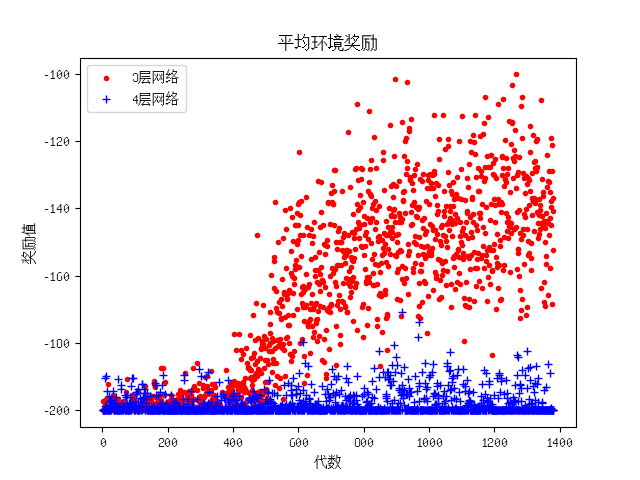
\includegraphics[width=0.6\textwidth]{sim_myenv_reward.png}
        \caption{浅层神经网络和深层神经网络的平均环境奖励曲线}
            \label{simenv_reward}
        \end{figure}

观察图\ref{simlsh_reward}中所示的基于局部敏感哈希的计数奖励可以发现,浅层网络的基于局部敏感哈希的计数奖励与深层网络的相差不多,甚至在200代附近深层网络反而获得了更高的奖励。

        \begin{figure}
        \centering
        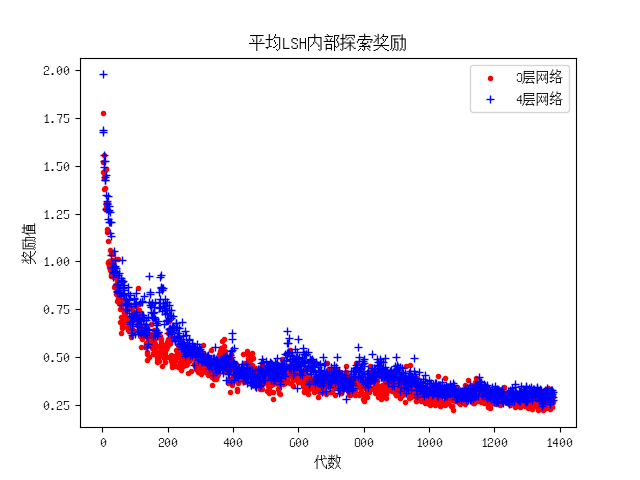
\includegraphics[width=0.6\textwidth]{sim_myenv_lsh_reward.png}
        \caption{浅层网络和深层网络的基于局部敏感哈希的平均计数奖励曲线}
            \label{simlsh_reward}
        \end{figure}
而仿真时间奖励则能比基于局部敏感哈希的计数奖励更好地反映策略的好坏,如图\ref{simsim_reward}所示,仿真时间奖励在900代之后浅层网络要比深层网络更高,这与环境奖励的趋势吻合,表明仿真时间奖励不仅具有任务无关的鼓励智能体探索的能力,还能帮助智能体在探索之后策略泛化到给定开放任务中。

        \begin{figure}
        \centering
        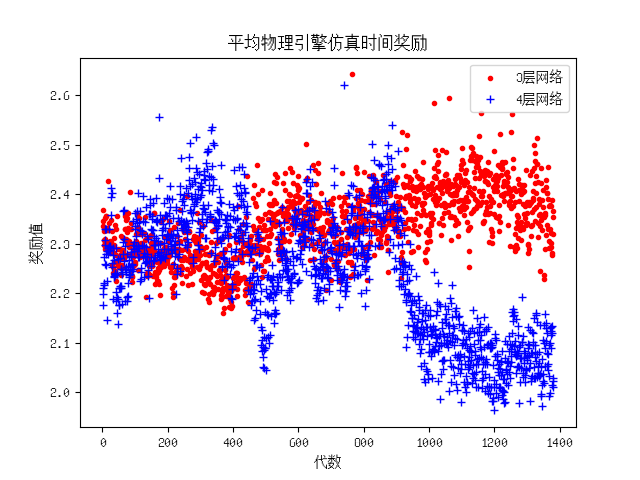
\includegraphics[width=0.6\textwidth]{sim_myenv_sim_reward.png}
        \caption{浅层网络和深层网络的平均仿真时间奖励曲线}
            \label{simsim_reward}
        \end{figure}
图\ref{simsuc_rate}中的成功率变化与环境奖励的变化趋势相似,这和在其他实验中观察到的一致。

        \begin{figure}
        \centering
        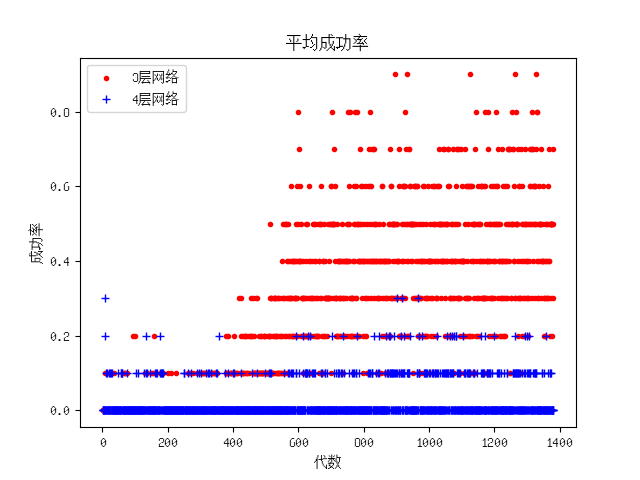
\includegraphics[width=0.6\textwidth]{sim_myenv_suc_rate.png}
        \caption{浅层网络和深层网络平均任务目标成功率曲线}
            \label{simsuc_rate}
        \end{figure}
在对深层网络的梯度进行观测时,可以观察到演员网络中的梯度快速地减小至0,这意味着发生了梯度消失,如果使用残差网络、层归一化或进行谱归一化,则有可能进一步提高性能。
